\chapter{Greedy Algorithms}

\emph{Greedy} algorithms build up a solution piece by piece, always choosing the next piece that offers the most obvious and immediate benefit. Although such an approach can be disastrous for some computational tasks, there are many for which it is optimal. Our first example is that of minimum spanning trees

\ex{}{Minimum Spanning Trees}

\textit{ Sol. }

\ex{}{Huffman encoding}

\textit{ Sol. }

To encode a message, we need to know how to decode it. This means that we need to know the code for each character. The code for each character is a binary string, and the codes for different characters must be distinct. \\

In general, how do we optimaly encode our message without loosing any information? \\

Let us consider the following example. Suppose we have a message consisting of the characters $A$, $B$, $C$, and $D$, with frequencies 70, 3, 20, and 37 million, respectively. We want to encode the message using the fewest bits possible.

\begin{center}
	\begin{tabular}{|c|c|}
		\hline
		\textbf{Symbol} & \textbf{Frequency} \\
		\hline
		$A$             & 70 million         \\
		\hline
		$B$             & 3 million          \\
		\hline
		$C$             & 20 million         \\
		\hline
		$D$             & 37 million         \\
		\hline
	\end{tabular}
\end{center}

In general how do we find the optimal tree, given the frequencies $f_1, f_2, \ldots, f_n$ of the characters that we want to encode?

\begin{align*}
	\text{Cost of a tree } T & = \sum_{i=1}^{n} f_i \cdot \text{depth of }i \text{th symbol in the tree} \\
\end{align*}

\textbf{Huffman's Algorithm}
Huffman's algorithm is a greedy algorithm that constructs an optimal prefix code called a Huffman code. The algorithm builds the tree in a bottom-up manner, starting with the leaves and combining two nodes at a time until the root is formed. The algorithm uses a priority queue to store the nodes of the tree. The priority queue is implemented as a min-heap. The algorithm works as follows:

\begin{algorithmic}
	\State \textbf{Huffman}($f_1, f_2, \ldots, f_n$)
	\State $Q \gets$ a priority queue of the characters with their frequencies \\
	\For{$i = 1$ to $n$}{
		\State Insert $f_i$ into $Q$
	} \\
	\For{$i = 1$ to $n-1$}{
		\State Create a new node $z$
		\State $z.left \gets x \gets$ Extract-Min($Q$)
		\State $z.right \gets y \gets$ Extract-Min($Q$)
		\State $z.freq \gets x.freq + y.freq$
		\State Insert $z$ into $Q$
	} \\
	\State \textbf{return} the root of the tree
\end{algorithmic}

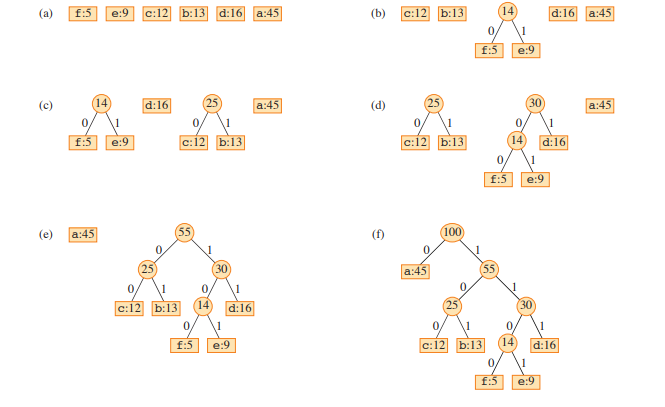
\includegraphics{HuffmanAlgorithm.png} 
\ex{}{Interval Scheduling}

\textit{ Sol. }


